\documentclass{article}
\usepackage[utf8]{inputenc}
\usepackage{mathtools}
\usepackage{pgfplots}
\usepackage{natbib}
\usepackage{graphicx}
\usepackage{amsmath}
\usepackage{amssymb}
\usepackage{amsfonts}
\usepackage{natbib}
\usepackage{minted}
\usepackage[a4paper,margin=1in,footskip=0.25in]{geometry}
\allowdisplaybreaks

\title{CSE546 Machine Learning HW1 - A}
\author{Bobby Deng | 1663039 | dengy7 }
\date{15 April 2020}



\begin{document}
\maketitle


\section{A.0}
\subsection{In your own words, describe what bias and variance are? What is bias-variance trade-off?}

In class, we have derived that the total variability is composed by three parts: irreducible error, bias and variance. Irreducible error is the lowest error that our model can get. Bias is how much our model is deviated from the true model. When the model is two simple, it is more likely to deviate largely from the model. When the model is too complex and fits all training data points. There would not be any bias at all. Variance is basically the variance of the model, when model is a horizontal line, there is no variance at all. But if the model is too complex, the geometry representation of the model becoming too zigzag, and this is where the variance tends to be very big.  
The bias-variance trade-off is saying that we need to find a balance point where testing error is at the lowest point. Testing error is presented as an u shape, so ideally we want to find the model that produces the testing error at the bottom of the u shape curve.

\subsection{What happens to bias and variance when the model complexity increases/decreases?}
When complexity increase, bias decrease, variance increase. When complexity decrease, bias increase, variance decrease.
Bias will be monotonically decrease and finally fits all training data points. Variance will be monotonically increase. 

\subsection{True or False: The bias of a model increases as the amount of training data available increases.}

False, bias dose not depend on the amount of training data points.

\subsection{True or False: The variance of a model decreases as the amount of training data available increases.}

True, the variance do depend on the amount of training data. 

\subsection{True or False: A learning algorithm will generalize better if we use less features to represent our data.}

False, we want enough useful and good predictors in the modes. The quality of predictor and coefficients determined how good our model might be. And less feature will not be better to present the ground truth model.

\subsection{To get better generalization, should we use the train set or the test set to tune our hyper-parameters?}

We should use train set to train the model and get hyper-parameters. We must not use any testing data in getting the hyper-parameters.
\subsection{True or False: The training error of a function on the training set provides an overestimate of the true error of that function.}

False, since we saw in both practice and theory that the training error is always lower than the testing error, in expectation. And when we train out model, our based model are generated by minimizing the error on training data. So it is an optimistic/underestimated estimation of the true function. 

\section*{A.1}
Use MLE to estimate $\lambda$ in Poisson Distribution.
\subsection*{a.}

\begin{subequations}
\begin{align*}
P(x|\lambda) & = \frac{e^{-\lambda}\lambda^{x}}{x!} \\
P(x_1, x_2, x_3, x_4, x_5|\lambda) 
& = \prod^{n}_{i=1}\frac{e^{-\lambda}\lambda^{x_i}}{x_i!} \text{ (Where n = 5.)} \\
\hat{\lambda}_{MLE} & = \arg\max_{\lambda} (P(x_1, x_2, x_3, x_4, x_5|\lambda) ) \\
& = \arg\max_{\lambda} (\prod^{n}_{i=1}\frac{e^{-\lambda}\lambda^{x_i}}{x_i!}) \\
& = \arg\max_{\lambda} ln(\prod^{n}_{i=1}\frac{e^{-\lambda}\lambda^{x_i}}{x_i!}) \\
& = \arg\max_{\lambda} \sum_{i=1}^{n} ln(\frac{e^{-\lambda}\lambda^{x_i}}{x_i!} ) \\
& = \arg\max_{\lambda} \sum_{i=1}^{n} (lne^{-\lambda}+ln\lambda^{xi}-ln(xi!)) \\
& = \arg\max_{\lambda}  (-n\lambda + ln\lambda*\sum_{i=1}^{n}xi + \sum_{i=1}^{n}ln(xi!)) \\
& \text{Then set the derivative to 0.} \\
0 & = \frac{d}{d\lambda} (-n\lambda + ln\lambda*\sum_{i=1}^{n}xi + \sum_{i=1}^{n}ln(xi!)) \\
& = -n + \frac{1}{\lambda} \sum_{i=1}^{n} xi + 0 \\
n & = \frac{1}{\lambda} \sum_{i=1}^{n} xi \\
\hat{\lambda}_{MLE} & = \frac{1}{n} \sum_{i=1}^{n} xi , n = 5.\\
\end{align*} 
\end{subequations}


\subsection*{b.}
\begin{subequations}
\begin{align*}
	\hat{\lambda}_{MLE} & = \arg\max_{\lambda} (P(\mathcal{D}|\lambda))                   \\
	                    & =  \arg\max_{\lambda} (P(x_1, x_2, x_3, x_4, x_5, x_6|\lambda)) \\
	                    & = \frac{1}{n} \sum_{i=1}^{n} xi , n = 6.
\end{align*}
\end{subequations}


\subsection*{c.}

For $\lambda $ after 5, $\hat{\lambda}_{MLE} = (2+0+1+1+2)/5 = \frac{6}{5}$. \newline
For $\lambda$ after 6, $\hat{\lambda}_{MLE} = (2+0+1+1+2+4)/6 = \frac{5}{3}$. \newline

So, we can see the result that the outlier has a big effect on the estimation.



\section*{A.2 German tank problem}
From the problem, we know that the serial of number came from a uniform distribution with $[0,\theta]$.

\[ 
f(x_i) = \begin{cases}
\frac{1}{\theta}  & \text{for $0\le x_i \le \theta$.}  \\
0 & \text{Otherwise.}
\end{cases}
\]

We can derive the MLE with uniform distribution.

\begin{subequations}
\begin{align*}
\hat{\theta}_{MLE} & = \arg\max_{\theta} (P(\mathcal{D}|\theta))                   \\
& =  \arg\max_{\theta} (\prod^{n} \frac{1}{\theta}) \\
& = \arg\max_{\theta} ln(\prod^{n} \frac{1}{\theta}) \\
& = \arg\max_{\theta} ln( \frac{1}{\theta^n}) \\
& = \arg\max_{\theta} -n ln(\theta) \\
\frac{d(ln(L(\theta)))}{d\theta} & = -n/\theta
\end{align*}
\end{subequations}

We can not set the derivative to zero in this particular problem since $\theta$ is impossible to be infinity. So here, the only thing we can do is let $\theta$ to be as large as it could be. We can not arbitrages assign value to $\theta$. What we can do is to assign the biggest X we have observed to $\theta$.  \newline

\[\hat{\theta} = max(x_1, \dots, x_n)\]



\section*{A.3}
\subsection*{a.}

\[ E_{train}[\hat{\epsilon}_{train}(f)] = E[ \frac{1}{N_{train}} \sum_{(x,y)\in S_{train}} (f(x)-y)^2 ] \]

\[ E_{train}[\hat{\epsilon}_{train}(f)] = \frac{N_{train}}{N_{train}} E[(f(x)-y)^2]\]

\[ E_{train}[\hat{\epsilon}_{train}(f)] = E[(f(x)-y)^2] =  \epsilon (f)\]
Since data from train and test are draw iid, the expectation for $(f(x)-y)^2$ should be the same.
\[E_{test}[\hat{\epsilon}_{test}(f)]  = \frac{N_{test}}{N_{test}} E[(f(x)-y)^2] = E[(f(x)-y)^2] =  \epsilon (f)\]
So,
\[E_{train}[\hat{\epsilon}_{train}(f)] = E_{test}[\hat{\epsilon}_{test}(f)] = \epsilon (f)\]


\subsection*{b.}
No, the equation is not generally true, because the estimator we got from training is by minimizing the training error. It is not able to be general enough to describe the true model.  
\subsection*{c.}
From the hint we know that,
\[
E_{train,test}[\hat{\epsilon}_{test}(\hat{f}_{train})]
= \sum_{f\in \mathcal{F}} E_{test}[\hat{\epsilon}_{test}(f)]  \mathbb{P}_{train}(\hat{f}_{train}=f)
\]
From a., we know that $ E_{train}[\hat{\epsilon}_{train}(f)] =  E_{test}[\hat{\epsilon}_{test}(f)]$. \newline
So, \[ = \sum_{f\in \mathcal{F}} E_{train}[\hat{\epsilon}_{train}(f)]  \mathbb{P}_{train}(\hat{f}_{train}=f) \]
Since $\hat{\epsilon}_{train}(\hat{f}) \le \hat{\epsilon}_{train}(f)$:

\[ \sum_{f\in \mathcal{F}} E_{train}[\hat{\epsilon}_{train}(\hat{f})]  \mathbb{P}_{train}(\hat{f}_{train}=f) \le \sum_{f\in \mathcal{F}} E_{train}[\hat{\epsilon}_{train}(f)]  \mathbb{P}_{train}(\hat{f}_{train}=f) \]

\[ \sum_{f\in \mathcal{F}} E_{train}[\hat{\epsilon}_{train}(\hat{f})]  \mathbb{P}_{train}(\hat{f}_{train}=f) \le  E_{train,test}[\hat{\epsilon}_{test}(\hat{f}_{train})] \]
Because $\sum_{f\in \mathcal{F}} \mathbb{P}_{train}(\hat{f}_{train}=f) = 1$:
\[ E_{train}[\hat{\epsilon}_{train}(\hat{f})] \sum_{f\in \mathcal{F}} \mathbb{P}_{train}(\hat{f}_{train}=f) \le  E_{train,test}[\hat{\epsilon}_{test}(\hat{f}_{train})] \] 

\[
E_{train}[\hat{\epsilon}_{train}(\hat{f}_{train})] \le
E_{train,test}[\hat{\epsilon}_{test}(\hat{f}_{train})]
\]


\section*{A.4}

\begin{minted}[mathescape,linenos,obeytabs=true,tabsize=2]{python}

import numpy as np


#-----------------------------------------------------------------
#  Class PolynomialRegression
#-----------------------------------------------------------------

class PolynomialRegression:

def __init__(self, degree=1, reg_lambda=1E-8):
	"""
	Constructor
	"""
	self.theta = None
	self.regLambda = reg_lambda
	self.degree = degree
	self.mean = None
	self.std = None

def polyfeatures(self, X, degree):
	"""
	Expands the given X into an n * d array of polynomial features of
	degree d.
	
	Returns:
	A n-by-d numpy array, with each row comprising of
	X, X * X, X ** 3, ... up to the dth power of X.
	Note that the returned matrix will not include the zero-th power.
	
	Arguments:
	X is an n-by-1 column numpy array
	degree is a positive integer
	"""
	outputX = X[:]
	for i in range(2, degree + 1):
		outputX = np.hstack((outputX,X**i))
	return outputX


def fit(self, X, y):
	"""
	Trains the model
	Arguments:
	X is a n-by-1 array
	y is an n-by-1 array
	Returns:
	No return value
	Note:
	You need to apply polynomial expansion and scaling
	at first
	"""
	
	X = self.polyfeatures(X, self.degree)
	# standardization
	self.mean = np.mean(X, axis=0)
	self.std = np.std(X, axis=0)
	X = (X - self.mean) / self.std
	n = len(X)
	# add 1s column
	X_ = np.c_[np.ones([n, 1]), X]
	n, d = X_.shape
	reg_matrix = self.regLambda * np.identity(d )
	reg_matrix[0, 0] = 0
	self.theta = np.linalg.pinv((X_.T @ X_) + reg_matrix) @ (X_.T @ y)
	print(self.theta)

def predict(self, X):
	"""
	Use the trained model to predict values for each instance in X
	Arguments:
	X is a n-by-1 numpy array
	Returns:
	an n-by-1 numpy array of the predictions
	"""
	
	n = len(X)
	X = self.polyfeatures(X, self.degree)
	X = (X - self.mean) / self.std
	# add 1s column
	X_ = np.c_[np.ones([n, 1]), X]
	# predict
	return X_ @ self.theta


#-----------------------------------------------------------------
#  End of Class PolynomialRegression
#-----------------------------------------------------------------

\end{minted}

When lambda is 0:

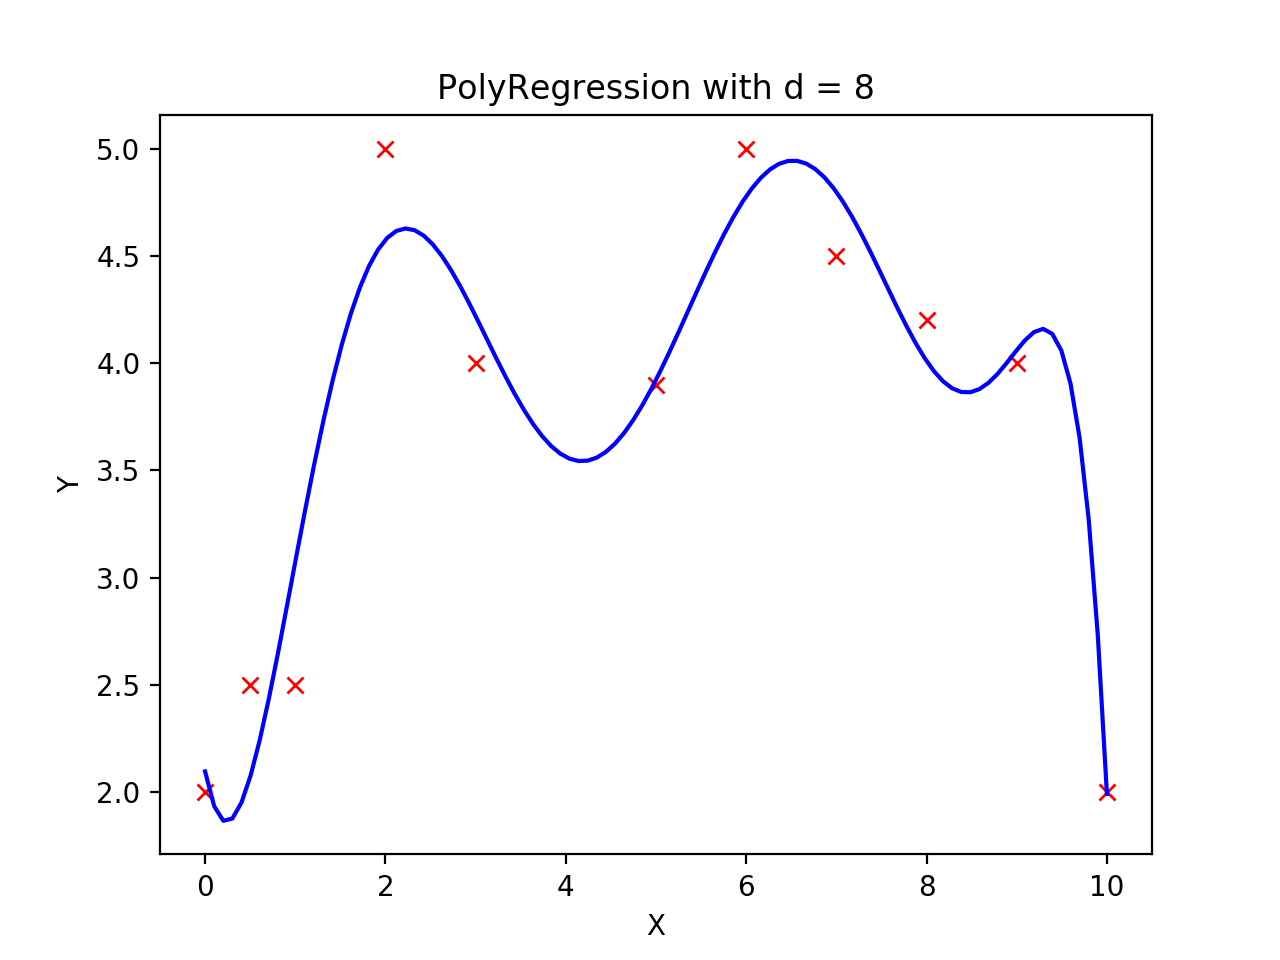
\includegraphics[width=5cm, height=4cm]{A4_0.png}

When lambda is 0.0001:

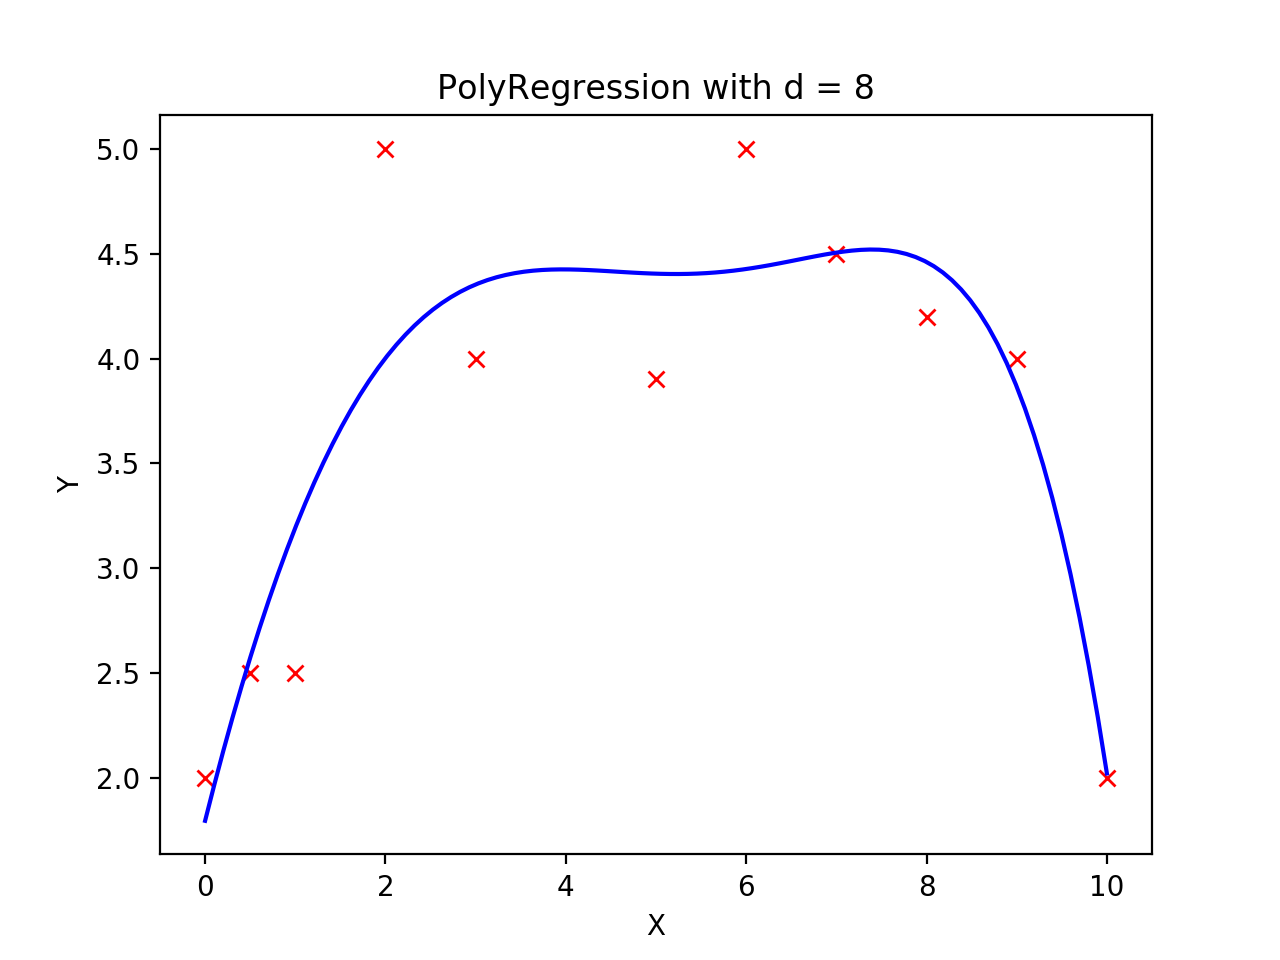
\includegraphics[width=5cm, height=4cm]{A4_0_0001.png}

When lambda is 0.01:

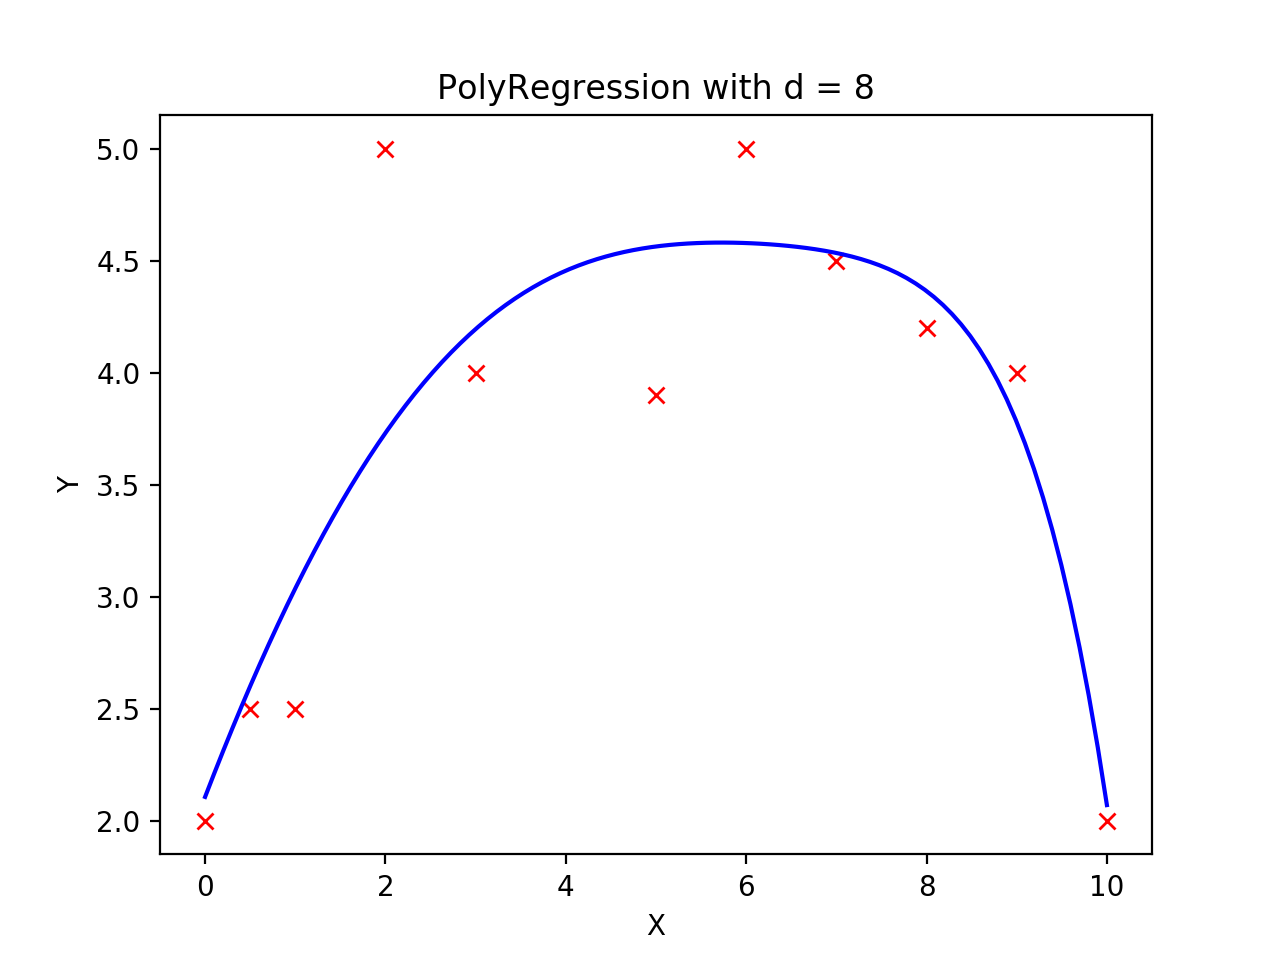
\includegraphics[width=5cm, height=4cm]{A4_0_01.png}

When lambda is 0.1:

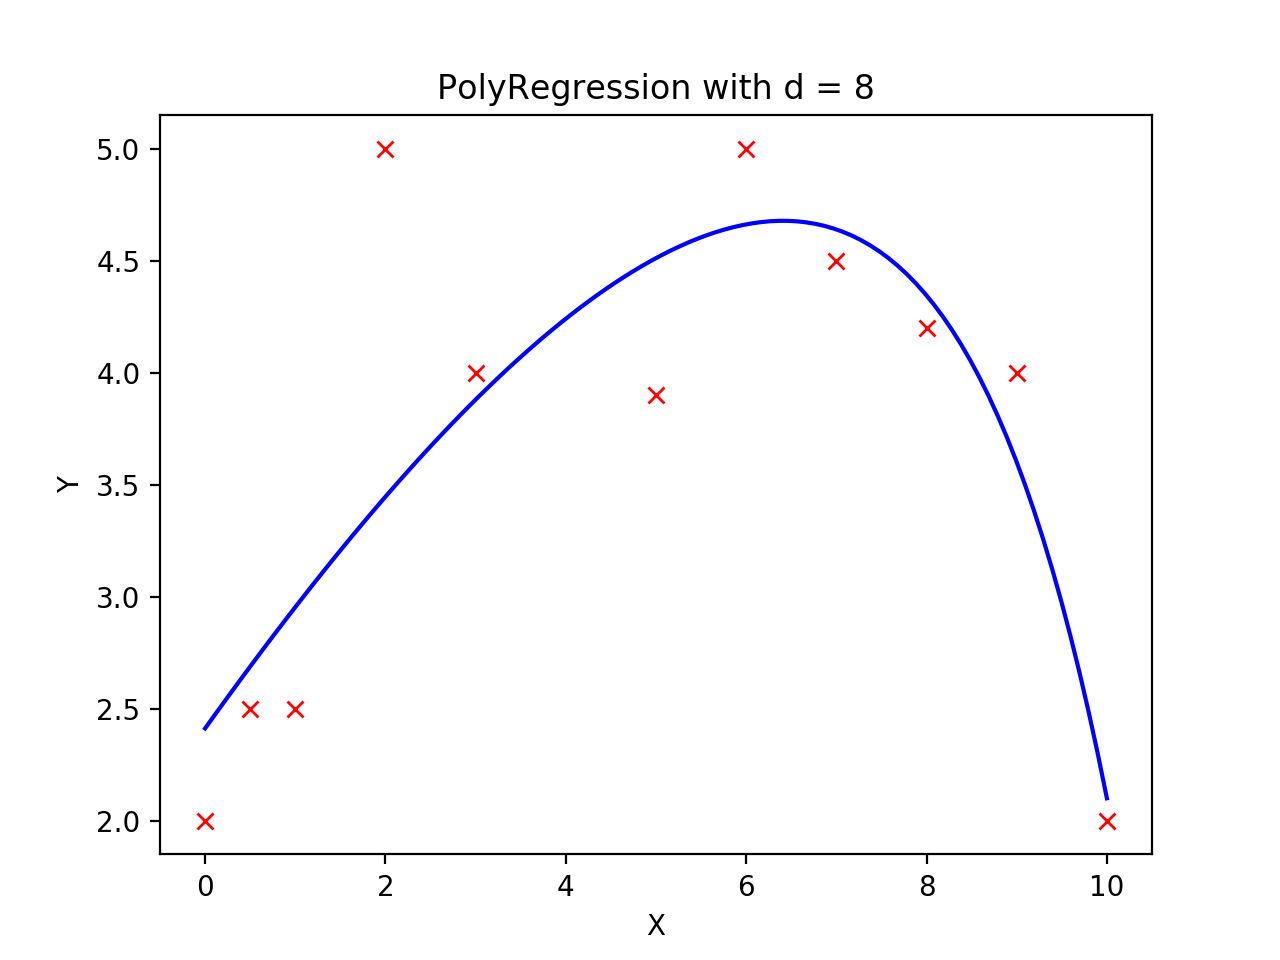
\includegraphics[width=5cm, height=4cm]{A4_0_1.png}

From the graph, we can see that when lambda increase out model gets smoother. And the model tends to be simpler. And the weight tends to be smaller.

\section*{A.5}

\begin{minted}[mathescape,linenos,obeytabs=true,tabsize=2]{python}
def learningCurve(Xtrain, Ytrain, Xtest, Ytest, reg_lambda, degree):
"""
Compute learning curve

Arguments:
Xtrain -- Training X, n-by-1 matrix
Ytrain -- Training y, n-by-1 matrix
Xtest -- Testing X, m-by-1 matrix
Ytest -- Testing Y, m-by-1 matrix
regLambda -- regularization factor
degree -- polynomial degree

Returns:
errorTrain -- errorTrain[i] is the training accuracy using
model trained by Xtrain[0:(i+1)]
errorTest -- errorTrain[i] is the testing accuracy using
model trained by Xtrain[0:(i+1)]

Note:
errorTrain[0:1] and errorTest[0:1] won't actually matter, since we start displaying the learning curve at n = 2 (or higher)
"""
n = len(Xtrain)

errorTrain = np.zeros(n)
errorTest = np.zeros(n)

for i in range(3, n+1):
print("i = ", i, " Degree= ", degree, " lambda: ", reg_lambda)
model = PolynomialRegression(degree, reg_lambda)
model.fit(Xtrain[:i], Ytrain[:i])

trainPredicted = model.predict(Xtrain[:i])
singleErrorFromTrain = np.mean((trainPredicted- Ytrain[:i])**2)
errorTrain[i-1] = singleErrorFromTrain

test_predicted = model.predict(Xtest[:i])
singleErrorFromTest = np.mean((test_predicted - Ytest[:i])**2)
errorTest[i-1] = singleErrorFromTest

return errorTrain, errorTest
\end{minted}

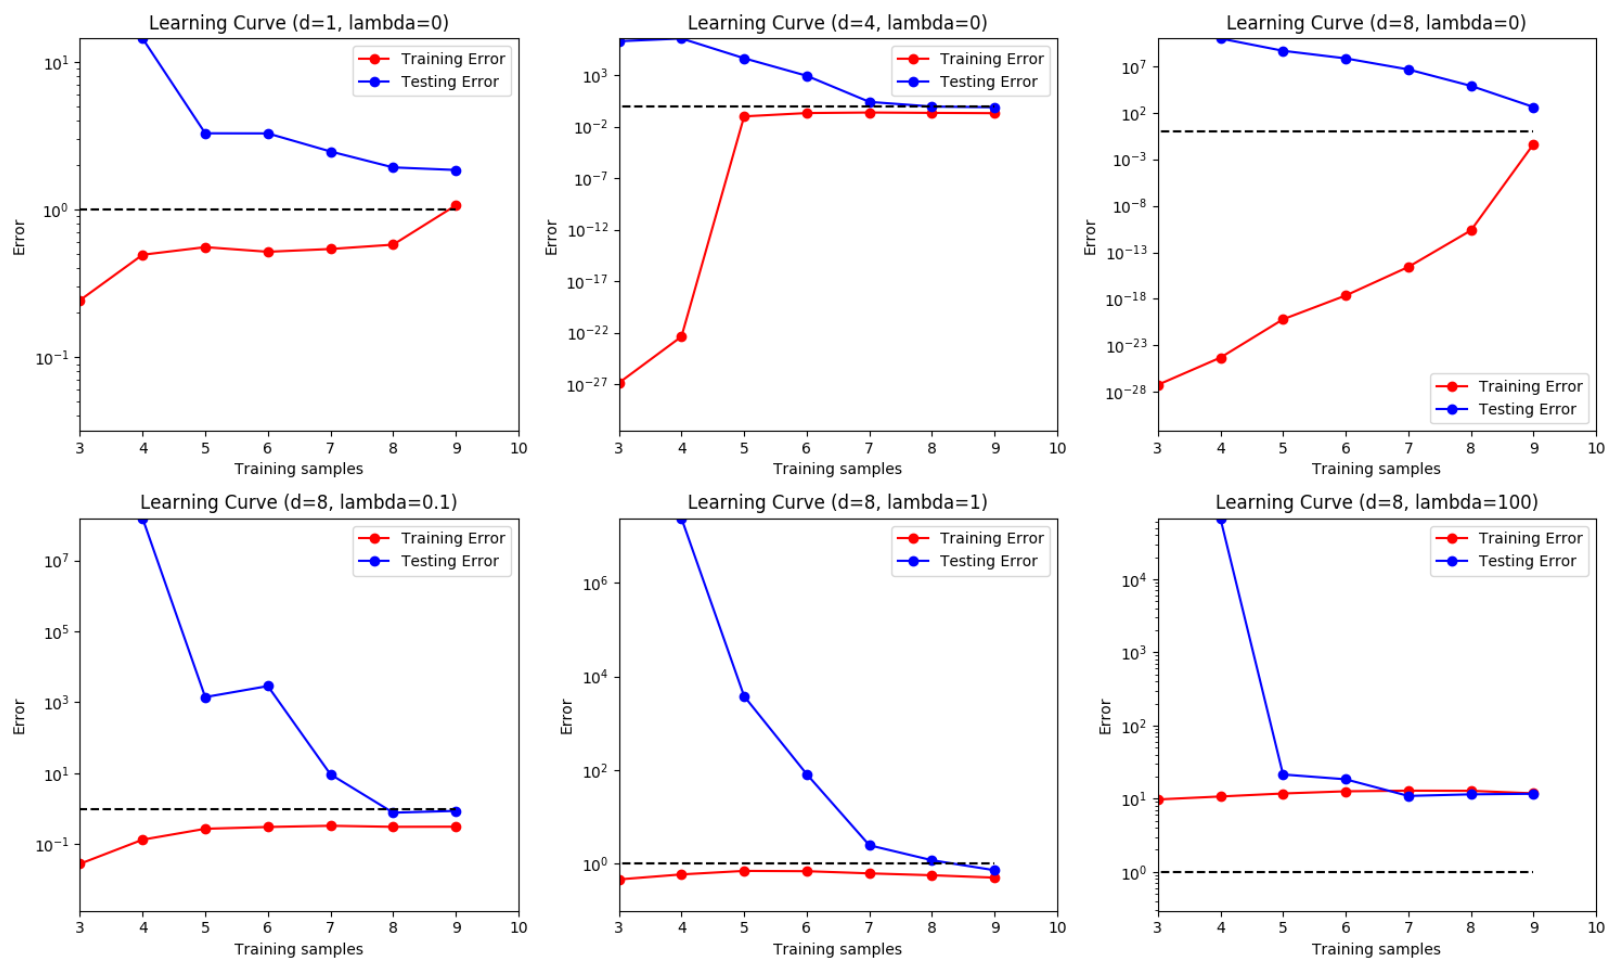
\includegraphics[width=12cm, height=8cm]{A5_1.png}




\section*{A.6}

\subsection*{a.}
From the problem we know that:
\[ \sum_{i=0}^{n} || W^T x_i - y_i ||^2_2 + \lambda||W||^2_F = \sum_{j=0}^{k} \Big[ ||Xw_j - Ye_j||^2 + \lambda||w_j||^2\Big] \]
Let:
\[ A =  \sum_{j=0}^{k} \Big[ ||Xw_j - Ye_j||^2 + \lambda||w_j||^2\Big] \]
Take derivative:
\[   \frac{\partial A}{\partial w_j} = \sum_{j=0}^{k} 2X^T\big[ Xw_j - Ye_j \big] +2\lambda w_j \]
Set derivative to 0 to find minimum,
\[ 0 = \sum_{j=0}^{k} 2X^T\big[ Xw_j - Ye_j \big] +2\lambda w_j \]

\[ 0 = \sum_{j=0}^{k} X^TXw_j +\lambda w_j - X^TYe_j \]

\[ \sum_{j=0}^{k} (X^TX + \lambda I)w_j = \sum_{j=0}^{k} X^TYe_j\]


Here, $X^T \in \mathbb{R}^{n \times d}$, $Y^T \in \mathbb{R}^{n \times k}$, $w_j \in \mathbb{R}^{d \times 1}$, $x_i \in \mathbb{R}^{d \times 1}$, $y_i \in \mathbb{R}^{k \times 1}$, $\lambda \in \mathbb{R}$, $e_j \in \mathbb{R}^{k \times 1}$, let's write it in matrix form:
\[ (X^TX + \lambda I)\hat{W} = X^TY \]
\[ \hat{W} = (X^TX + \lambda I)^{-1}X^TY \]
\subsection*{b.}

\begin{minted}[mathescape,linenos,obeytabs=true,tabsize=2]{python}
import mnist
import numpy as np

mndata = mnist.MNIST("./python-mnist/data/")
X_train, labels_train = map(np.array, mndata.load_training()) 
X_test, labels_test = map(np.array, mndata.load_testing()) 
X_train = X_train/255.0
X_test = X_test/255.0

# Train function
def train(X,y,lam):
	n, d = X.shape
	y = np.eye(10)[y] # put y into a one hot encoding matrix
    reg_matrix = self.regLambda * np.identity(d )
    reg_matrix[0, 0] = 0
    self.theta = np.linalg.pinv((X_.T @ X_) + reg_matrix) @ (X_.T @ y)
	return W

def predict(W, X_new):    
	return (X_new @ W_hat).argmax(axis=1)

# Compute weights
W_hat = train(X_train, labels_train, lam = 0.00001)
# Computed predicted training label
predicted_train = predict(W=W_hat, X_new=X_train)
# Compute predicted testing label
predicted = predict(W=W_hat, X_new=X_test)
# Compute error rate for both training and testing
train_error_rate = 1 -( sum(predicted_train == labels_train) / len(labels_train))
test_error_rate = 1 - (sum(predicted == labels_test) / len(labels_test))
print("Training Accuracy is: ", train_error_rate)
print("Testing Error Rate is: ", test_error_rate)
#Training Error is:  0.14806666666666668
#Testing Error Rate is:  0.14659999999999995
\end{minted}

















\end{document}
